\section{Presential Laboratory}
\label{sec:Presencial}

In this last laboratory assigment, due to some changes in the university directives, one student from each group was allowed to participate in a laboratory session, in person. This change was very positive beacause although we could simulate and learn from our experiences in the Ngspice software, being able to see and feel (and possibly even fry) the components brings another meaning and perspective to the work we have been doing throughout the semester and motivates the students to explore and pursue careers in the eletronics field. Therefore we thank the professor for the time it took to make these labs possible and for sparking our curiosity for this field. Here are some of the pictures/registers we were able to take during the lab assigment:  

\begin{figure}[H] \centering
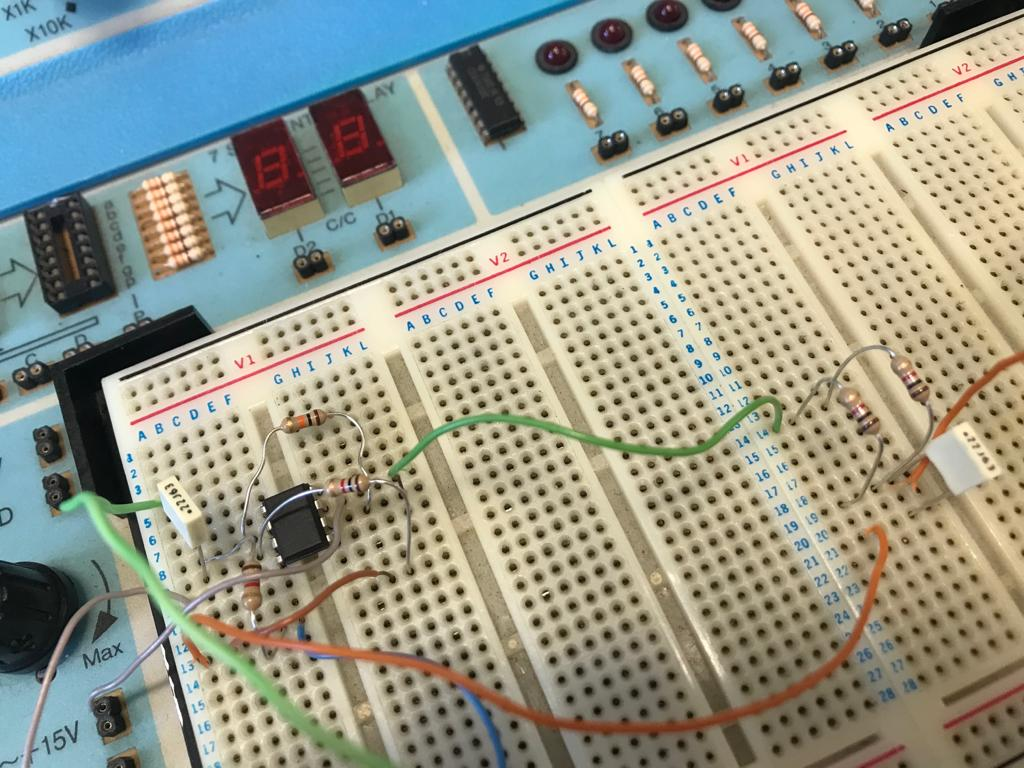
\includegraphics[width=0.95\linewidth]{try1_diagram.jpeg}
%\vspace{-10cm}
\caption{First attempt: everything connected, does it work? Let's see...}
\label{fig:t11}
\end{figure}

  
\begin{figure}[H] \centering
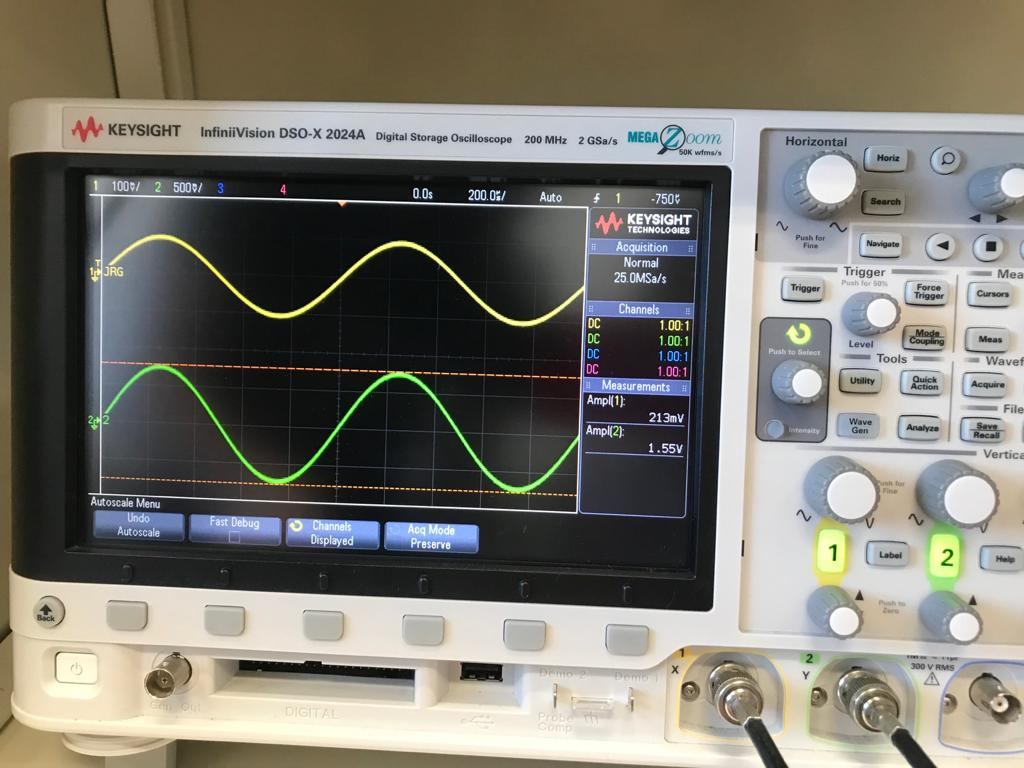
\includegraphics[width=0.5\linewidth]{try1_results.jpeg}
%\vspace{-1cm}
\caption{First attempt: It works! Even if with a clearly insufficient gain $Gain = \frac{1.55}{0.213}=7.277$. But at least everything seem to be going smoothly.}
\label{fig:t12}
\end{figure}


\begin{figure}[H] \centering
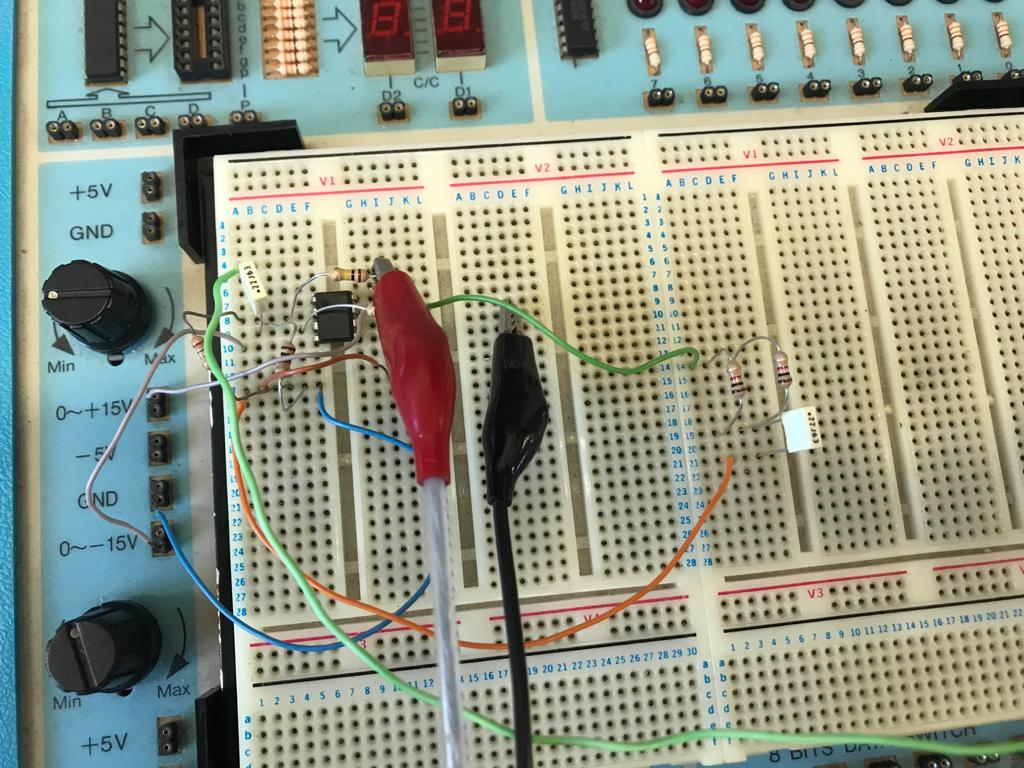
\includegraphics[width=0.5\linewidth]{try2_diagram.jpeg}
\caption{Second attempt: let's try to improve the gain, and hope the OPAMP doesn't saturate. (Basically we played around with the resistors). The jumper cables were because of some electrical noise which was coming from Ground feedback loops (the voltage source, breadboard, and osciloscope all had their grounds connected). We had no idea this could de problematic! The solution was to trade in the grounded connector cable for these jumpers and leave the ground "hanging".}
\label{fig:t21}
\end{figure}
%\vspace{-3cm}

\begin{figure}[H] \centering
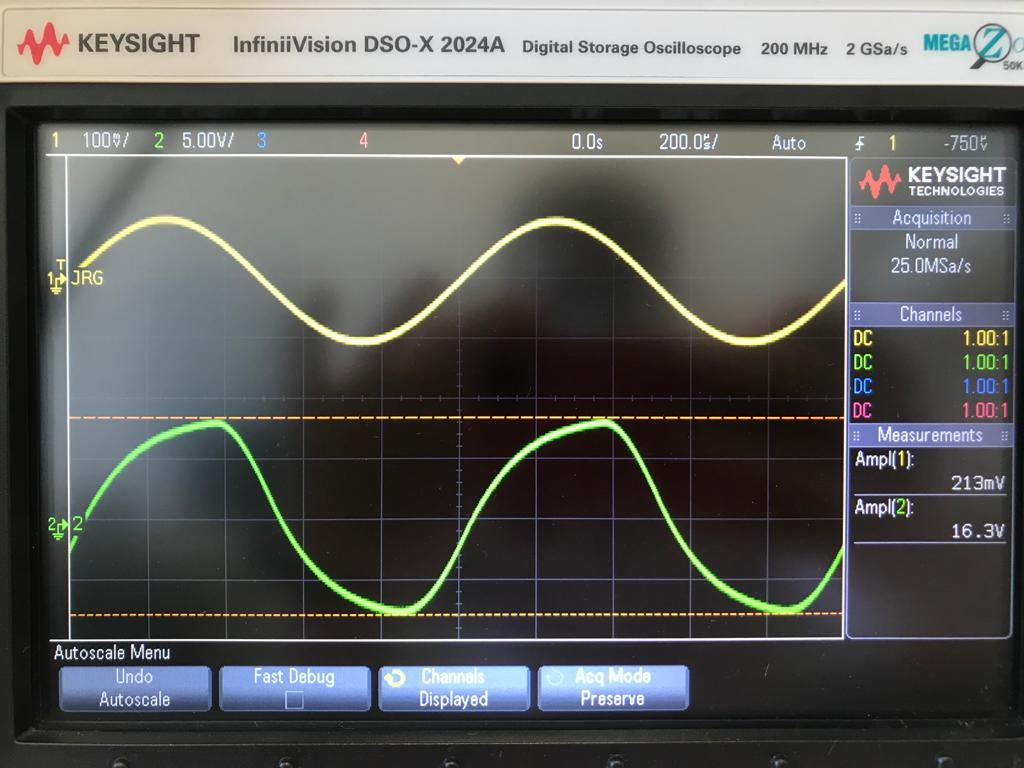
\includegraphics[width=0.5\linewidth]{saturated.jpeg}
\caption{Oh no! It saturated! We will have to reduce the 213mV input amplitude until it is not saturating anymore and we can have a clear reading of the gain.}
\label{fig:t3}
\end{figure}
%\vspace{-3cm}


\begin{figure}[H] \centering
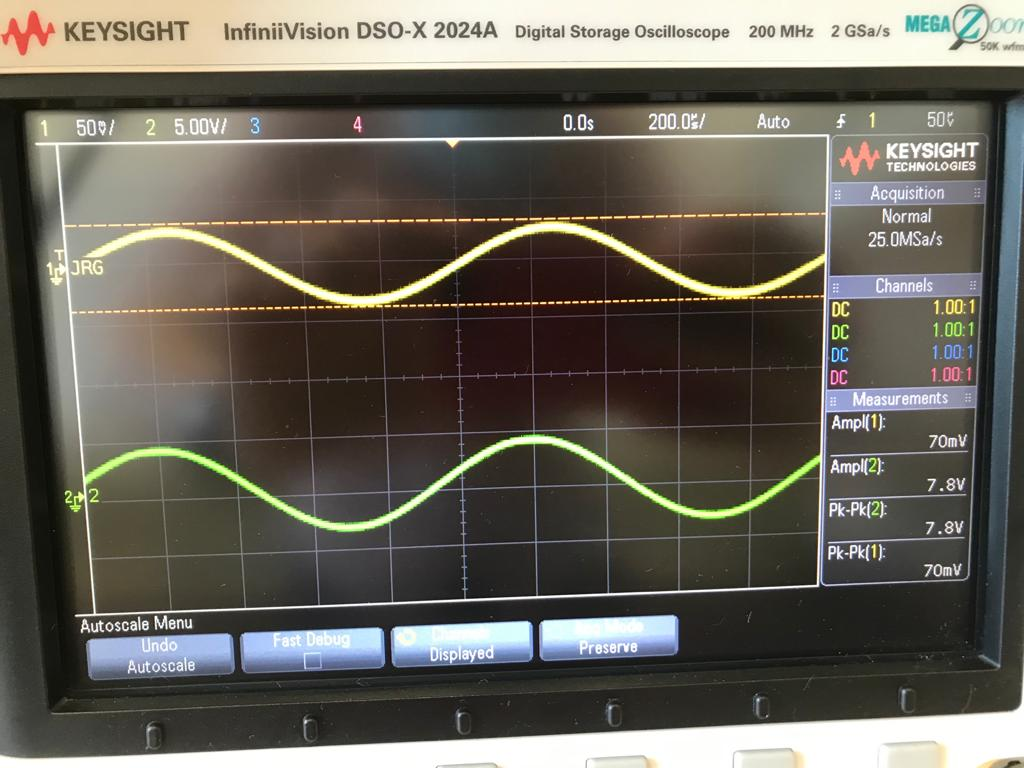
\includegraphics[width=0.6\linewidth]{try2_results.jpeg}
\caption{Second attempt: Eureka! No more saturation. $Gain = \frac{7.8}{0.07}=111.43$. All right, we admit this might be a tad bit over 40dB but it is quite close with the limited components we have. With some extra time we will improve this in Ngspice! But even so this is a good starting point for our simulation attempts.}
\label{fig:t22}
\end{figure}
\vspace{-3cm}


\pagebreak
